\documentclass[10pt, a5paper]{article}
\usepackage{pdfpages}
\usepackage{parallel}
\usepackage[T2A]{fontenc}
\usepackage{ucs}
\usepackage[utf8x]{inputenc}
\usepackage[polish,english,russian]{babel}
\usepackage{hyperref}
\usepackage{rotating}
\usepackage[inner=2cm,top=1.8cm,outer=2cm,bottom=2.3cm,nohead]{geometry}
\usepackage{listings}
\usepackage{graphicx}
\usepackage{wrapfig}
\usepackage{longtable}
\usepackage{indentfirst}
\usepackage{array}
\newcolumntype{P}[1]{>{\raggedright\arraybackslash}p{#1}}
\frenchspacing
\usepackage{fixltx2e} %text sub- and superscripts
\usepackage{icomma} % коскі ў матэматычным рэжыме
\PreloadUnicodePage{4}

\newcommand{\longpage}{\enlargethispage{\baselineskip}}
\newcommand{\shortpage}{\enlargethispage{-\baselineskip}}

\def\switchlang#1{\expandafter\csname switchlang#1\endcsname}
\def\switchlangbe{
\let\saverefname=\refname%
\def\refname{Літаратура}%
\def\figurename{Іл.}%
}
\def\switchlangen{
\let\saverefname=\refname%
\def\refname{References}%
\def\figurename{Fig.}%
}
\def\switchlangru{
\let\saverefname=\refname%
\let\savefigurename=\figurename%
\def\refname{Литература}%
\def\figurename{Рис.}%
}

\hyphenation{admi-ni-stra-tive}
\hyphenation{ex-pe-ri-ence}
\hyphenation{fle-xi-bi-li-ty}
\hyphenation{Py-thon}
\hyphenation{ma-the-ma-ti-cal}
\hyphenation{re-ported}
\hyphenation{imp-le-menta-tions}
\hyphenation{pro-vides}
\hyphenation{en-gi-neering}
\hyphenation{com-pa-ti-bi-li-ty}
\hyphenation{im-pos-sible}
\hyphenation{desk-top}
\hyphenation{elec-tro-nic}
\hyphenation{com-pa-ny}
\hyphenation{de-ve-lop-ment}
\hyphenation{de-ve-loping}
\hyphenation{de-ve-lop}
\hyphenation{da-ta-ba-se}
\hyphenation{plat-forms}
\hyphenation{or-ga-ni-za-tion}
\hyphenation{pro-gramming}
\hyphenation{in-stru-ments}
\hyphenation{Li-nux}
\hyphenation{sour-ce}
\hyphenation{en-vi-ron-ment}
\hyphenation{Te-le-pathy}
\hyphenation{Li-nux-ov-ka}
\hyphenation{Open-BSD}
\hyphenation{Free-BSD}
\hyphenation{men-ti-on-ed}
\hyphenation{app-li-ca-tion}

\def\progref!#1!{\texttt{#1}}
\renewcommand{\arraystretch}{2} %Іначай формулы ў матрыцы зліпаюцца з лініямі
\usepackage{array}

\def\interview #1 (#2), #3, #4, #5\par{

\section[#1, #3, #4]{#1 -- #3, #4}
\def\qname{LVEE}
\def\aname{#1}
\def\q ##1\par{{\noindent \bf \qname: ##1 }\par}
\def\a{{\noindent \bf \aname: } \def\qname{L}\def\aname{#2}}
}

\def\interview* #1 (#2), #3, #4, #5\par{

\section*{#1\\{\small\rm #3, #4. #5}}

\def\qname{LVEE}
\def\aname{#1}
\def\q ##1\par{{\noindent \bf \qname: ##1 }\par}
\def\a{{\noindent \bf \aname: } \def\qname{L}\def\aname{#2}}
}


\begin{document}

\title{Heartbeat: построение отказоустойчивого кластера}%\footnote{Текст данных и последующих тезисов, кроме специально оговоренных случаев, доступен под лицензией Creative Commons Attribution-ShareAlike 3.0}

\author{Юрий Волкович\footnote{Минск, Беларусь}}
\maketitle

\begin{abstract}
Report presents an approach to build a cluster for web server, as well as author's personal experience and some interesting decisions in this matter.
\end{abstract}

В рамках данной темы под кластером понимается система высокой доступности,
т.е. построенная с расчетом того, что она продолжает работать безотказно,
даже если какая-то ее часть выходит из строя.

Heartbeat "--- продукт проекта Linux-HA \cite{Volkovich1}, позволяющий реализовать механизм безотказной работы отдельных частей кластера.

\subsection*{Задача}

Решаемая задача заключалась в построении отказоустойчивого кластера из двух web-серверов, которые могут моментально заменить друг друга в случае выхода из строя одного из них. Сервер предназначен для авторизации на таких сайтах, как irr.ru, job.ru и др., аудитория которых насчитывает несколько миллионов пользователей в сутки, поэтому его значимость для компании достаточно велика.

\subsection*{Используемое ПО}

Законченное решение было построено на следующем наборе программных продуктов:

\begin{itemize}
  \item heartbeat (поднимает виртуальный ip и проверяет доступность соседнего сервера);
  \item monit \cite{Volkovich2} (следит за правильной работой демонов, обслуживающих сайт);
  \item web-сервер (связка nginx \cite{Volkovich3}, php-fpm \cite{Volkovich4}, mongodb \cite{Volkovich5}, \linebreak memcache \cite{Volkovich6}).
\end{itemize}

\subsection*{Схема взаимодействия демонов}

\begin{figure}[h!]
  \centering
  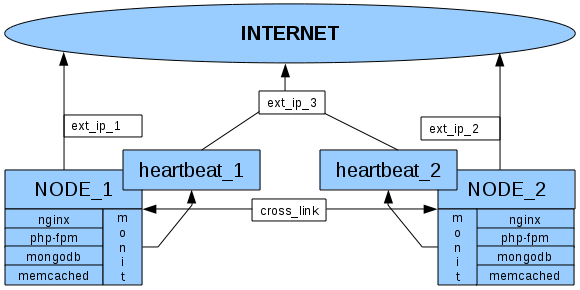
\includegraphics[width=11cm]{01_2012_heartbeat}
  \label{fig:Volkovich1}
\end{figure}

Для начала поднимаются два сервера NODE\_1 и NODE\_2, на которых запущена работающая версия сайта. Затем на оба сервера подключается heartbeat. Он должен <<держать>> виртуальный адрес virt\_ip и следить за доступностью соседнего сервера, а при сбое на текущем --- передавать virt\_ip heartbeat'у соседнего сервера. Однако, этого не достаточно для полного отслеживания того, работает ли сайт, поскольку heartbeat не обладает возможностью проверять работоспособность базы данных mongodb либо других используемых сервисов. Эти задачи можно делегировать демону monit, настроенному для проверки того, работают ли все необходимые демоны.

На данном этапе конфигурация, в принципе, является завершенной, и если какой-то из демонов на мастер-сервере <<упадет>>, обслуживание сайта немедленно будет перенаправлено на второй сервер. Но, как показала практика, и этого оказывается недостаточно в случае, когда демон работает, но при этом выдает неверные данные, либо просто зависает, захватив все наличные ресурсы. Для решения данной проблемы нами было написано несколько небольших скриптов, которые запускаются по cron'у и проверяют такие параметры, как репликацию в memcached и mongodb, отдачу http-трафика через php-fpm и др. менее значительные нюансы. И в случае, если проверка не проходит, в скрипте (как и в monit) выполняется команда hb\_standby, которая заставляет heartbeat принудительно отдать virt\_ip на slave-сервер, если таковой имеется.

\subsection*{Конфигурация демонов}

Ниже приведены ключевые параметры, использованные нами при конфигурировании:

\subsubsection*{heartbeat}

\begin{itemize}
  \item haresources
%\end{itemize}
\begin{verbatim}
    passport1.pronto.ru IPaddr::194.87.222.180/27/eth0 nginx
\end{verbatim}
%\begin{itemize}
  \item ha.cf
%\end{itemize}
\begin{verbatim}
    debugfile /var/log/ha-debug
    logfile /var/log/ha-log
    logfacility local0
    keepalive 2
    deadtime 30
    warntime 10
    initdead 120
    udpport 694
    ucast eth1 192.168.0.2
    auto_failback off
    node passport1.pronto.ru passport2.pronto.ru
    ping_group ping_nodes 8.8.8.8
    respawn hacluster /usr/lib/heartbeat/ipfail
    deadping 30
    use_logd yes
    debug 1
\end{verbatim}
\end{itemize}
\subsubsection*{monit}

\begin{itemize}
  \item monitrc
%\end{itemize}
\begin{verbatim}
    check process nginx
    with pidfile "/var/run/nginx.pid"
    start program = "/etc/init.d/nginx start"
    stop program = "/etc/init.d/nginx stop"
    group www
\end{verbatim}
\end{itemize}
\subsection*{Тестирование}

При проверке работоспособности системы мы использовали следующие способы нарушения работоспособности сайта:

\begin{itemize}
  \item моментальное отключение питания на мастер-ноде;
  \item падение интерфейса на мастер-ноде;
  \item падение любого из демонов, обслуживающего сайт;
  \item нарушение репликации memcached и mongodb.
\end{itemize}

Результатом любого из перечисленных событий являлось

\begin{itemize}
  \item моментальное переключение ip-адреса сайта на соседний сервер;
  \item отправка администраторам уведомлений обо всех событиях.
\end{itemize}


\begin{thebibliography}{9}

\bibitem{Volkovich1} \url{http://www.linux-ha.org}

\bibitem{Volkovich2} \url{http://mmonit.com/monit}

\bibitem{Volkovich3} \url{http://sysoev.ru/nginx}

\bibitem{Volkovich4} \url{http://php-fpm.org}

\bibitem{Volkovich5} \url{http://www.mongodb.org}

\bibitem{Volkovich6} \url{http://memcached.org}

\end{thebibliography}

\end{document}




